\documentclass[12pt]{report}

\usepackage[top=3cm,bottom=3cm,left=3cm,right=3cm]{geometry}
\usepackage{graphicx}
\usepackage{float}
\usepackage{setspace}
\usepackage{fancyhdr}

\setlength{\parindent}{0pt}
\onehalfspacing

\pagestyle{fancy}
\fancyhf{}
\fancyfoot[C]{\thepage}
\renewcommand{\headrulewidth}{0pt}

\begin{document}

% -------------------- TITLE PAGE --------------------
\thispagestyle{empty}
\begin{center}
    \vspace*{1.2cm}

    {\Large\textbf{A Report on AegisOps: Applied Cyber Defense and\\
    Cryptography Operations Suite}}\\[1.2cm]

    {\itshape A report submitted in partial fulfillment of the requirements\\
    for the award of the degree of}\\[2.1cm]

    {\large\textbf{by}}\\[0.7cm]

    \begin{tabular}{c c}
        \textbf{YELLANKI KRANTHI GIRI VENKATA CHARY} & \textbf{2420030539}
    \end{tabular}\\[1.2cm]

    \textbf{Dr.Jagan Mohan Reddy D}

    \vfill

    
\includegraphics[width=0.34\textwidth]{images/logo.png}\\[0.9cm]

    \textbf{KONERU LAKSHMAIAH EDUCATION FOUNDATION, BOWRAMPET}\\[0.45cm]
    \textbf{Hyderabad-500043, Telangana, India}\\[0.45cm]
    2026

    \vspace*{0.4cm}
\end{center}
\clearpage

% -------------------- PROJECT SUMMARY --------------------
\chapter*{About the Project}

\textbf{AegisOps} is an educational Cybersecurity and Cryptography Operations Suite developed for Active Learning Management Project--2 (ALM-2). It combines three security projects in one web dashboard. The frontend is developed using React and Vite, while the three backend services are developed using Python and Flask.

The first project, \textbf{AegisCrypt}, demonstrates public-key cryptography, RSA encryption and digital signatures, X.509 certificates, Diffie--Hellman key exchange, and Elgamal signatures. The second project, \textbf{NexusTunnel}, explains how TLS, SSH, and IPsec create secure communication channels. The third project, \textbf{Citadel Defense}, demonstrates firewall rules, a bastion host, intrusion detection, and statistical anomaly detection.

The main purpose of the project is to convert cybersecurity theory into an interactive practical demonstration. All three modules can be opened from a single dashboard, and all 13 supplied unit tests passed successfully.

\begin{figure}[H]
    \centering
    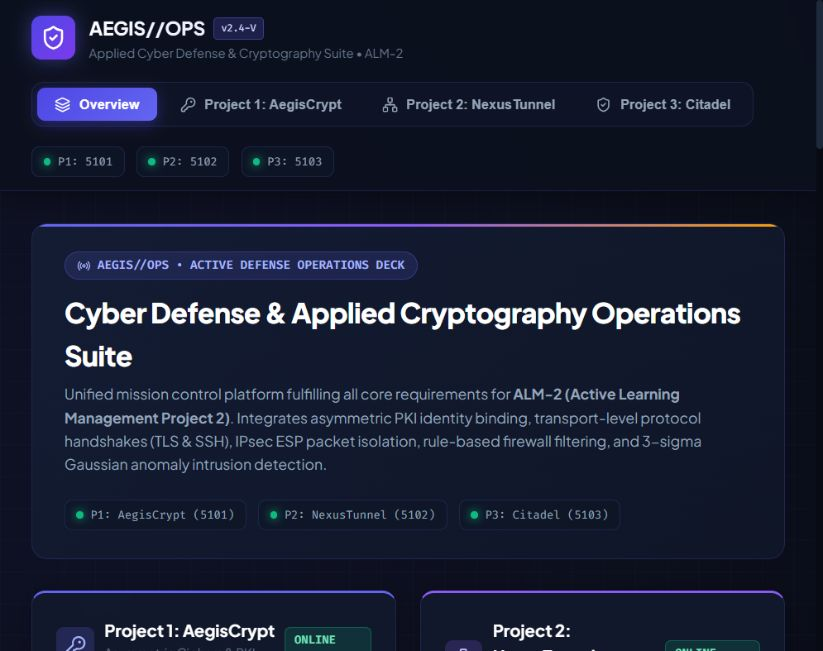
\includegraphics[width=\textwidth]{images/dashboard-overview.jpg}
    \caption{Unified AegisOps Dashboard}
\end{figure}

The dashboard displays the status of all three backend services and provides direct navigation to every security module.

\clearpage

% -------------------- PROJECT 1 --------------------
\chapter*{Project 1: AegisCrypt}

\begin{figure}[H]
    \centering
    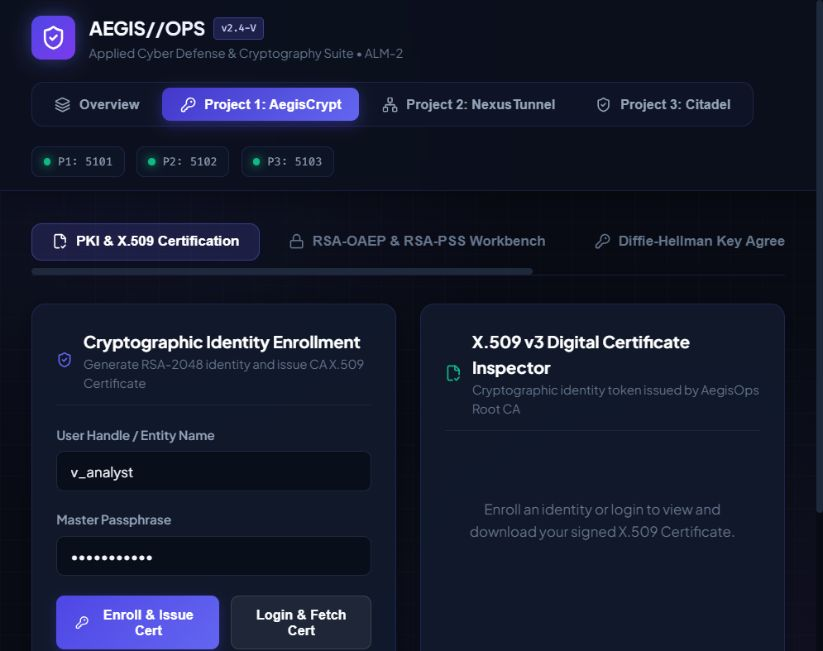
\includegraphics[width=\textwidth]{images/project1-aegiscrypt.jpg}
    \caption{AegisCrypt Cryptography and PKI Module}
\end{figure}

AegisCrypt is used to demonstrate user identity enrollment, RSA-2048 key generation, X.509 certificates, RSA-OAEP encryption, RSA-PSS signatures, Diffie--Hellman key exchange, and Elgamal signatures with SHA-512. It helps students understand confidentiality, authentication, integrity, and secure key exchange.

\section*{Main Features}
\begin{itemize}
    \item \textbf{User Authentication and PKI:} Registers users, generates RSA key pairs, and issues X.509 digital certificates that bind an identity to a public key.
    \item \textbf{RSA Encryption:} Uses RSA-OAEP with SHA-256 to encrypt and decrypt messages securely.
    \item \textbf{Digital Signatures:} Uses RSA-PSS to sign messages and verify their authenticity and integrity.
    \item \textbf{Diffie--Hellman Exchange:} Shows how Alice and Bob calculate the same shared secret without directly transmitting the secret.
    \item \textbf{Elgamal and SHA-512:} Hashes a message using SHA-512 and creates an Elgamal signature that can be verified using the public key.
\end{itemize}

\section*{Security Concepts Demonstrated}
This module explains confidentiality, integrity, authentication, non-repudiation, certificate-based trust, and secure key agreement. It also shows why secure padding and message hashing are important in modern cryptography.

\clearpage

% -------------------- PROJECT 2 --------------------
\chapter*{Project 2: NexusTunnel}

\begin{figure}[H]
    \centering
    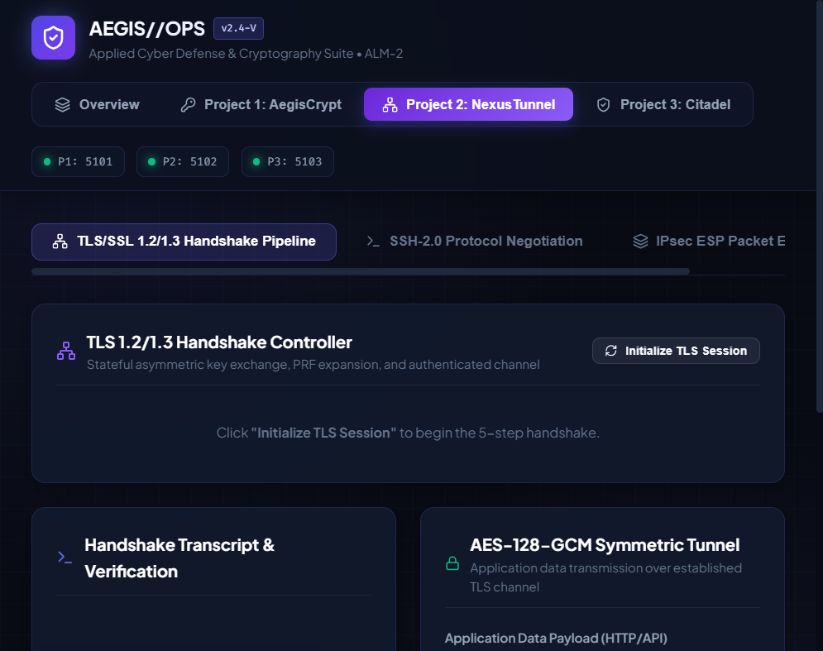
\includegraphics[width=\textwidth]{images/project2-nexustunnel.jpg}
    \caption{NexusTunnel Secure Communication Module}
\end{figure}

NexusTunnel visually explains secure network communication. It demonstrates the steps of a TLS handshake, encrypted data transfer using AES-GCM, SSH connection establishment, and the difference between IPsec ESP transport mode and tunnel mode.

\section*{Main Features}
\begin{itemize}
    \item \textbf{TLS Handshake:} Demonstrates Client Hello, Server Hello, certificate exchange, key generation, and Finished-message verification.
    \item \textbf{Encrypted Data Transfer:} Uses the generated symmetric session key with AES-128-GCM to protect application data.
    \item \textbf{SSH Connection:} Explains protocol negotiation, Diffie--Hellman key exchange, server authentication, user authentication, and secure shell creation.
    \item \textbf{IPsec ESP:} Displays the structure of an Encapsulating Security Payload packet and compares transport mode with tunnel mode.
\end{itemize}

\section*{Security Concepts Demonstrated}
This module demonstrates how encryption, authentication, key derivation, and integrity checking create a secure tunnel over an untrusted network. It also explains how TLS protects web traffic, SSH protects remote administration, and IPsec protects network packets.

\clearpage

% -------------------- PROJECT 3 --------------------
\chapter*{Project 3: Citadel Defense}

\begin{figure}[H]
    \centering
    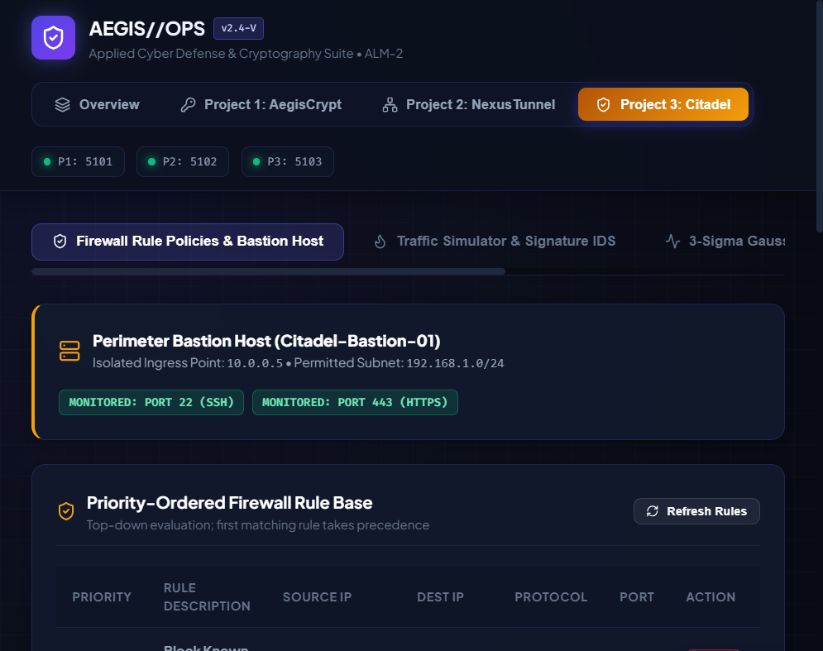
\includegraphics[width=\textwidth]{images/project3-citadel.jpg}
    \caption{Citadel Defense Firewall and IDS Module}
\end{figure}

Citadel Defense demonstrates priority-based firewall rules, a protected bastion host, packet inspection, and intrusion detection. It detects known attacks such as SSH brute force, Telnet usage, and port scanning, while a three-sigma model identifies unusual traffic increases.

\section*{Main Features}
\begin{itemize}
    \item \textbf{Firewall Rule Manager:} Creates and evaluates allow or block rules using source address, destination address, protocol, port, and priority.
    \item \textbf{Default-Deny Protection:} Blocks a packet when it does not match an approved allow rule.
    \item \textbf{Bastion Host:} Uses a controlled gateway for administrative access and reduces direct exposure of internal systems.
    \item \textbf{Rule-Based IDS:} Detects known patterns such as repeated SSH login failures, insecure Telnet traffic, and port scanning.
    \item \textbf{Anomaly Detection:} Uses the traffic mean and standard deviation to identify packet rates above the three-sigma threshold.
    \item \textbf{Threat Encyclopedia:} Provides short learning material about viruses, worms, attacks, and defensive measures.
\end{itemize}

\section*{Security Concepts Demonstrated}
This module explains network access control, defense in depth, attack detection, traffic monitoring, and the difference between signature-based and anomaly-based intrusion detection. It shows how prevention and detection can work together in one defensive system.

\end{document}
